\documentclass[aip, cp, amsmath, amssymb, reprint]{revtex4-2}

\usepackage{graphicx}
\usepackage{dcolumn}
\usepackage{bm}

\input{preamble/preamble}
\input{preamble/tikz}
\input{preamble/macros}


% ========================================= %
% LaTeX Template by Aditya K. Rao
% Contact at adi.rao@mail.utoronto.ca

% Change for each document [!!!]
\newcommand\course{PHY385}	% Course Code [!!!]txt
\newcommand\doctitle{Michael Interferometer} % Report Title [!!!]
\newcommand\firstauthorname{Aditya K. Rao}
\newcommand\firstauthorstdnum{Student Number: 1008307761}
\newcommand\firstauthoremail{adi.rao@mail.utoronto.ca}
%\newcommand\secondauthorname{Author Two}
%\newcommand\secondauthorstdnum{Student Number: 0000000000}
%\newcommand\secondauthoremail{report.author@mail.utoronto.ca}
\newcommand\advname{Boris Braverman\space} % Advisor Name [!!!]  
\newcommand\taname{Michael Sloan\space} % Advisor Name [!!!] 
\newcommand\lponename{Jack Wang\space}
\newcommand\lptwoname{Yiheng Wang\space}  
\newcommand{\location}{MP222} % Location [!!!]
% ========================================= %
 
% ============== EQUIPMENT ================ %

\newcommand{\oscope}{\texttt{DSOX1202G}\space}
\newcommand{\pdiode}{\texttt{DET36A2}\space}
\newcommand{\hene}{\texttt{HNLS008L}\space}

% ========================================= %



%\pagenumbering{gobble}
\usepackage{listings}

\renewcommand\lstlistingname{Code Reference}
\renewcommand\lstlistlistingname{Code Reference}
\usepackage{tikz}
\usetikzlibrary{patterns}

\usepackage{circuitikz}

%\addbibresource{references.bib}
\usepackage{lipsum}
\usetikzlibrary{calc}

\begin{document}
\onecolumngrid
\pagenumbering{arabic}
\title{\doctitle}
\author{\firstauthorname}
\email{\firstauthoremail}
\thanks{\firstauthorstdnum}

\author{\lponename}
\author{\lptwoname}

%\email{report.author@mail.utoronto.ca}
%\thanks{Student Number: 0000000000}
\affiliation{
University of Toronto \\
\location, 60 St. George Street, Toronto, Ontario M5S 1A7, Canada.% Force line breaks with \\ if necessary
}

\date{\today} %Put in date of submission [!!!]

\preprint{APS/123-QED}
\begin{abstract}
    An experiment was designed and attempted to build a Michaelson Interferometer and quantify the interferences patterns observed. The experiment was conducted using a \hene laser, beam splitter, and mirrors. The fringe contrast was calculated to be $0.5$.
\end{abstract}
    \maketitle
    %\tableofcontents 

    \lhead{\firstauthorname\vspace{0.1cm}}
    \chead{\textbf{\course} \\ \doctitle}
    \rhead{\textbf{Prof:} \advname \\ \textbf{TA:} \taname}
    \nocite{*}

    %\newpage
    \twocolumngrid
    \section{Introduction}
        Invented by Albert Abraham Michelson 1887 \cite{pwoptics}, the Michaelson Interferometer is a configuration of mirrors and beam splitters which can be used to quantify the interference patterns of light. It has been instrumental in the development of quantum mechanics and the theory of relativity. The Michaelson Interferometer is used in a variety of applications, including the measurement of the speed of light, the refutation of the existance of the ether, and the study of quantum mechanics.

        Michaelson Interferometers work on the basic principle of interference. In the experimental setup, a beam of light is split into two paths by a 50:50 beam splitter. The two beams are then reflected by mirrors and recombined at the beam splitter. The recombined beams interfere with each other, creating a pattern of light and dark fringes. The fringe contrast is a measure of the visibility of the fringes and is calculated using \eqref{eqn:fringeconstrast}.
    
        \begin{equation} \label{eqn:fringeconstrast}
            F = \dfrac{V_{\text{max}} - V_{\text{min}}}{V_{\text{max}} + V_{\text{min}}}
        \end{equation}

        Depending on the relative path difference, $d$, between the two reflected beams, there will be a time delay, $\tau$ defined by \eqref{eqn:timedelay} \cite{pwoptics}.

        \begin{equation} \label{eqn:timedelay}
            \tau = \dfrac{d}{c}
        \end{equation}            

        With the resultant intensity quantified by \eqref{eqn:intensity} \cite{pwoptics}.

        \begin{equation} \label{eqn:intensity}
            I = 2 I_0 \left[1 +  \cos(\omega t)\right]
        \end{equation}


    \section{Methodology}

        \begin{figure}[H]
            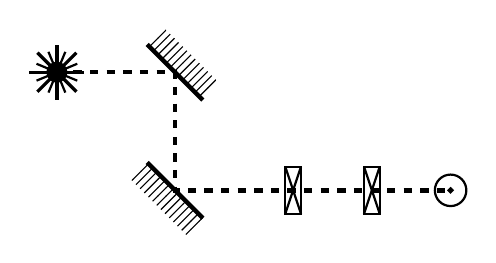
\begin{tikzpicture}
    \coordinate (L) at (0,0);
    \coordinate (M1) at (1.5,0);
    \coordinate (M2) at (1.5,-1.5);
    \coordinate (P1) at (3,-1.5);
    \coordinate (P2) at (4,-1.5);
    \coordinate (D) at (5,-1.5);

    % Laser Symbol
    \begin{scope}[scale=0.7]
        \draw[ultra thick, fill = black] (0,0) circle (0.15);
        \draw[rotate=0, very thick] (-0.5,0) -- (0.5,0);
        \draw[rotate=90, very thick] (-0.5,0) -- (0.5,0);
        \draw[rotate=45, very thick] (-0.5,0) -- (0.5,0);
        \draw[rotate=135, very thick] (-0.5,0) -- (0.5,0);

        \draw[rotate=22.5, thick] (-0.4,0) -- (0.4,0);
        \draw[rotate=67.5, thick] (-0.4,0) -- (0.4,0);
        \draw[rotate=112.5, thick] (-0.4,0) -- (0.4,0);
        \draw[rotate=157.5, thick] (-0.4,0) -- (0.4,0);
    \end{scope}


    % Mirror #1
    \begin{scope}[shift={(M1)}, rotate=-45]
        \draw[ultra thick] (-0.5,0) -- (0.5,0);
        \fill[pattern=north east lines] (-0.5,0) rectangle (0.5,0.30);
        %\coordinate (M1) at (0,-0.15);
    \end{scope}

    % Mirror #2
    \begin{scope}[shift={(M2)}, rotate=135]
        \draw[ultra thick] (-0.5,0) -- (0.5,0);
        \fill[pattern=north east lines] (-0.5,0) rectangle (0.5,0.30);
        %\coordinate (M2) at (0,-0.15);
    \end{scope}

    % Polarizer #1
    \begin{scope}[shift={(P1)}, scale=0.5]
        \draw[thick] (-0.2,0.6) rectangle (0.2,-0.6);
        \draw[thick] (-0.2,0.6) -- (0.2,-0.6);
        \draw[thick] (0.2,0.6) -- (-0.2,-0.6);
        %\coordinate (P1) at (0,0);
    \end{scope}

    % Polarizer #2
    \begin{scope}[shift={(P2)}, scale=0.5]
        \draw[thick] (-0.2,0.6) rectangle (0.2,-0.6);
        \draw[thick] (-0.2,0.6) -- (0.2,-0.6);
        \draw[thick] (0.2,0.6) -- (-0.2,-0.6);
        %\coordinate (P2) at (0,0);
    \end{scope}

    % Detector
    \begin{scope}[shift={(D)}, scale=0.5]
        \draw[thick] (0,0) circle (0.4);
        \draw[thick, fill=black] (0,0) circle (0.05);
        %\coordinate (D) at (0,0);
    \end{scope}

    % Laser Path
    \draw[ultra thick, dashed] (L) -- (M1) -- (M2) -- (P1) -- (P2) -- (D);
\end{tikzpicture}
            \caption{Figure}
        \end{figure}



    \section{Results \& Analysis}
        
    
    \section{Discussion}
    
    
    \section{Conclusion}



    % Line to seperate report content from acknowledgements and references
    \onecolumngrid
    \begin{center}
        \vspace{0.8cm}
        \noindent\rule{0.9\textwidth}{0.5pt}
    \end{center}
/home/adi/University/Physics/PHY385/Labs/Lab02/parta.csv
    \begin{acknowledgments}
        The work conducted by the other lab partners was instrumental in this lab. Thank you to \lponename and \lptwoname for their help in setting up the equipment and conducting the experiments. Additionally, thank you to the Teaching Assistant \taname and Professor \advname for their guidance and support.
    \end{acknowledgments}

\bibliography{references}

\appendix
\section{Appendix}
\subsection{Raw Data}

\subsection{Analysis Code}
\subsubsection{Toolkit}
\lstinputlisting{../toolkit.py}

\end{document}